\documentclass[10pt]{article}
\usepackage{mathtools}
\usepackage{amssymb}
\usepackage{amsthm}
\usepackage{hyperref}
\usepackage{graphicx}


\title{Particle Filter (assignment 1)}
\author{Yi Tian Xu\\260520039}


\begin{document}
\maketitle

\section{Initialization}
At the beginning, I create $n=400$ particles, each assigned with a random $x$ and $y$ coordinate from to the uniform distribution, and a random angle $\theta$ from to the Gaussian distribution. All weights are initialized with the inverse of the total number of particles. This can ensure that the initial hypothesis of the robot's position is not biased by regions that are more condense or by particles that have more weights. 

\section{Motion Model}
When the robot makes a move, each particle $s = (x, y, \theta)$ is replaced by a new particle $s' = (x', y', \theta')$ sampled from the distribution of $p(s'|u_{t-1}, s)$ where $u_{t-1}$ is the action taken at time $t-1$. I assumed that this distribution is Gaussian with mean and covariance matrix:
\begin{align*}
	&\mu = s + \delta \\ 
	&\Sigma = \begin{pmatrix}
				0.01 & 0.0 & 0.0 \\
				0.0. & 0.01 & 0.0 \\
				0.0 & 0.0 & 0.01  \end{pmatrix} 
\end{align*}
where $\delta = (\delta_x, \delta_y, \delta_{\theta})$ represent the values on the odometer when taking action $u_{t-1}$. This implies that $X$, $Y$, $\Theta$ are independent random variables distributed normally. 

The weight of the new particle is the same as the old one. 

\subsection{Design Decisions}
In a previous design, the covariance matrix was chosen to match the odometer's error, \texttt{odom\_error} as given in \texttt{lab.world} file. However, after doing some tests, it seems that arbitrary choices for the standard deviation that are consistent with the odometer's measurements are good enough to simulate the noise. 

\section{Sensor Model}
The weight of particles is updated based on the data that the robot receives with its laser sensor. To do so, simulations of the received data are done for each particle, and the ``distance" between each simulated data point with the true data point is used as the comparison method to calculate the new weight. 

Since the object \texttt{sensor\_msgs/LaserScan} in ROS has the data array sorted by the angle of the laser scan, I calculate the new weight as follows. Given a simulated sequence of ranges $R'_n = (r'_1, r'_2, \dots, r'_n)$ at the position of some particle $s$, and the true sequence $R_n = (r_1, r_2, \dots, r_n)$,
\begin{displaymath}
	p(r_i|s) = \exp\left(-\frac{\left(r'_i - r_i\right)^2}{l^2}\right)
\end{displaymath}
where $l$ is a constant. The new weight of particle $s$ is defined as
\begin{displaymath}
	w' = \frac{\alpha}{1-w} \sum_{i=1}^n p(r_i|s)
\end{displaymath}
where $w$ is the old weight and $\alpha$ is the normalization factor.

\subsection{Design Decisions}
For time efficiency, I tried to compare the minimum and maximum ranges between the simulated and true data before deciding to compare all the ranges. I proposed that if this comparison shows that there is a significant difference, i.e.: if the difference between minimum or maximum ranges is above a certain threshold, then I set the new weight to zero. However, the choice of the threshold was unclear. Moreover, in some circumstances, this heuristic wipes out many particles that are near the true position and allocates many new particles at some other places that happens to have similar minimum and maximum ranges but with different order. So I removed this heuristic. 

Probabilistically, it would make more sense if the new weight is defined as
\begin{displaymath}
	w' = \alpha p(R_n|s)w = \alpha p(r_1, \dots, r_n|s)w
\end{displaymath} 
Since $r_1, \dots, r_n$ are not independent, $p(r_1, \dots, r_n|s)$ can be difficult to calculate. So I use the sum of the individual probability instead, combined with $(1-w)^{-1}$ rather than $w$ to help avoiding serious underflow (as in the case when the weight sums up to zero). 

\section{Resampling}
As the weights keeps updating, it often happens that all but a few particles have weight close to zero. To avoid this degeneracy, I am using a resampling algorithm found in the paper by Arulampalam et al. in 2002 \cite[p. 180]{paper}. 

Consider the weight as a random variable $W$. In this algorithm, we first approximate the effective sample size, $N_{eff}$, like so
\begin{displaymath}
	N_{eff} = \frac{1}{1+Var(W)} \approx \frac{1}{\sum_{s}w^2}
\end{displaymath}
and we check if it is smaller than some threshold $N_T$. This indicate whether there's a severe degeneracy. If there is, we then we estimate the cumulative distribution function (CDF) of the weights using the weights themselves as probabilities. This can be easily done since the weights are already normalized in the sensor model. 

Defining a quantile $q_{\nu_i}$ to be the section in the CDF such that $p(W > w) < \nu_i$ for some value $w$. The algorithm chooses $n$ new particles such that there is at most $i$ particles with weight in quantile $q_{\nu_i}$, $\nu_i\in \{u +n^{-1}*(i-1)\}$, where $u$ is drawn from uniform distribution on the interval $[0, n^{-1}]$.

\subsection{Design Decisions}
The algorithm assign each of the new particles with the same position than the first particle whose weight is above the smallest quantile that the new particle corresponds to. I thought that, in the case there is a lot of degeneracy, it may happen that some particle is so heavy that it is the only closest representative above some consecutive quantiles. So I used Gaussian distribution centered at the old particle's position to add more dispersion.
 
\section{Estimate Update}
As the density of the particles now describes the significance of the region where they are allocated to, I defined the new estimate to be the sample mean.
\begin{displaymath}
	\bar{s} = \frac{1}{n}\sum_{s} s
\end{displaymath}
Since I assumed that $X$, $Y$, $\Theta$ are independent, the covariance matrix is a diagonal matrix. I used the sample variance to estimate it. 

\subsection{Design Decisions}
As $n$ is large, the sample variance becomes
\begin{displaymath}
	\hat{\sigma}_x = \frac{1}{n-1}\sum_{s}(x-\bar{x})^2 \approx \frac{1}{n}\sum_{s}(x-\bar{x})^2
\end{displaymath}
and likewise for $\hat{\sigma}_y$ and $\hat{\sigma}_\theta$. So to simplify the computation, I used the formula on the right hand side to approximate the estimate. 

Furthermore, since $\bar{s}$ must be known before computing the variance, I used the previous estimate to avoid making another loop in the program. 

\section{Performance}
My implementation is able to estimate the robot's location with a high standard deviation within a reasonable time. Occasionally the estimated position matches closely to the robot's true location and orientation. 

When particles converges to a region on the map, they may disperse again when the robot quickly moves to another location. 

\begin{figure}[ht!]
\centering
\advance\leftskip-3cm
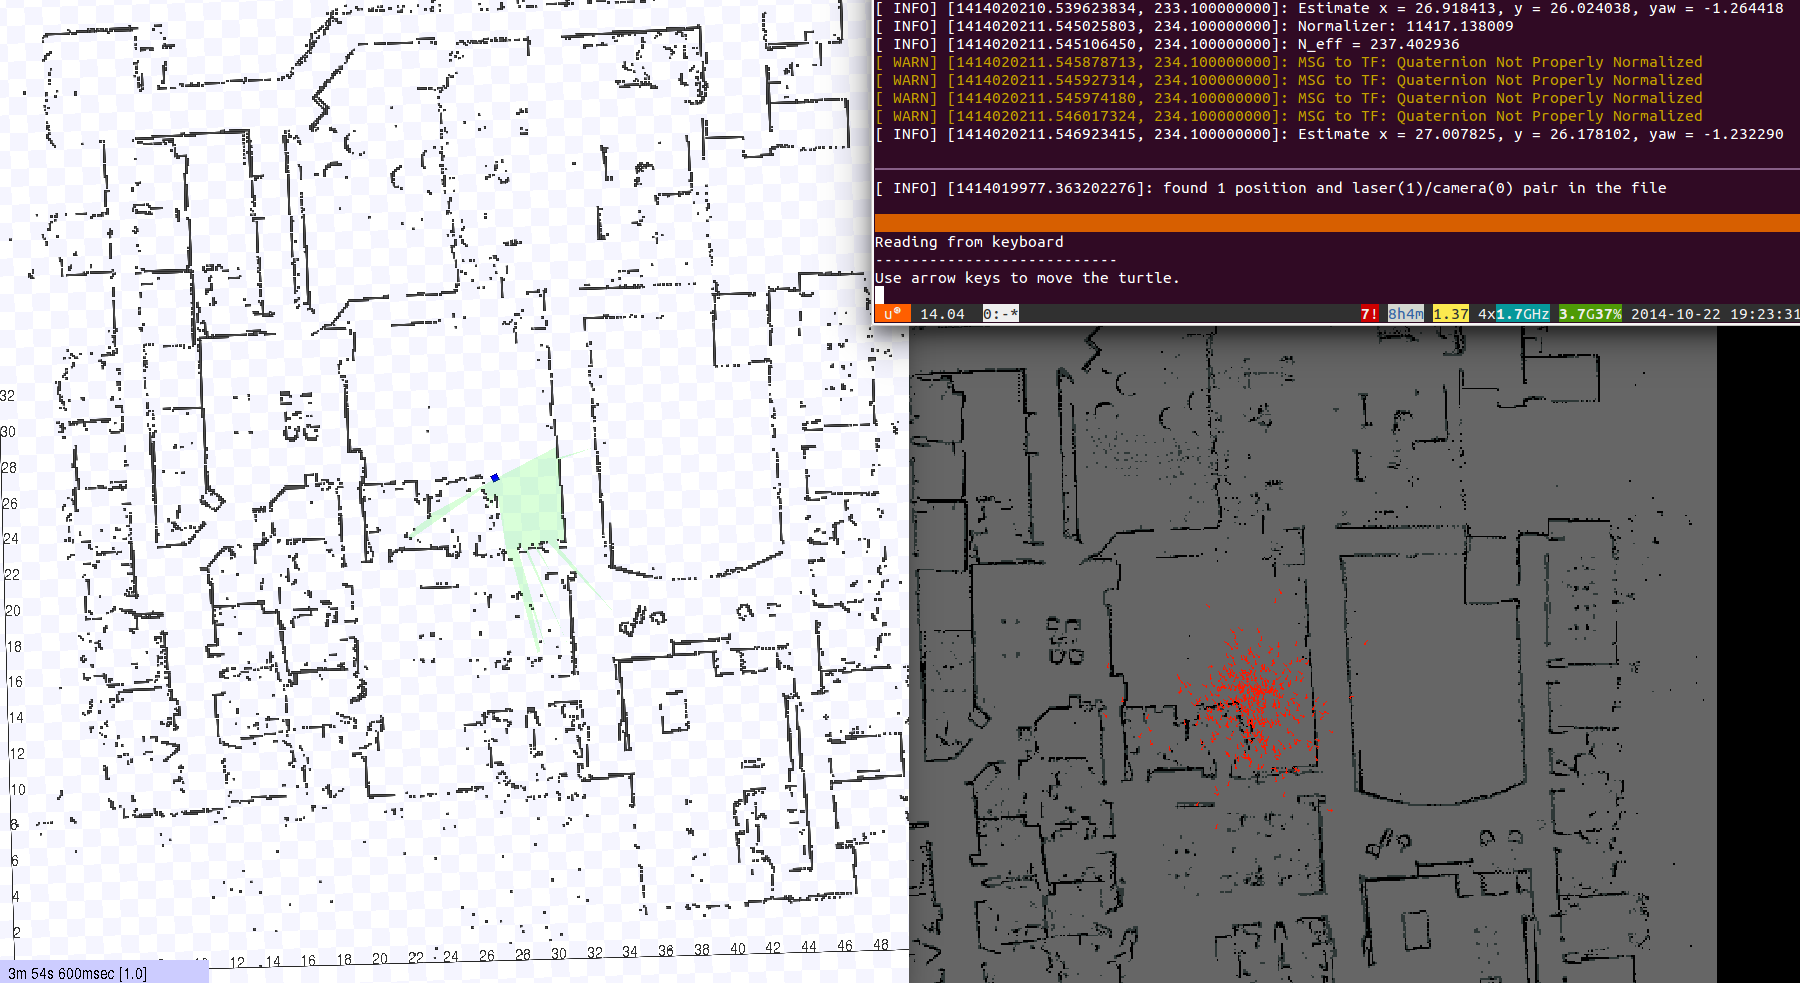
\includegraphics[width=180mm]{pic.png}
\caption{The particles converging at $s \approx (27,26,-1.23)$.}
\label{figCir1}
\end{figure}

\section{Improvements}
Often, the particles may converge to a region on the map that is not the true location of the robot. This happens when there are many locations scattered on the maps that look similar for the robot, resulting local maxima in the space of distribution functions of the particles. To jump out of those local maxima, we can consider adding random restart algorithm. 

Aside from adding more features, the choice for the number of particles ($n$), the noise in the motion model ($\Sigma$), the threshold for the effective sample size ($N_T$) and the constant in the sensor model ($l$) can be further explored and optimized to improve the performance of this algorithm. 


\begin{thebibliography}{9}

\bibitem{paper}
  M. Sanjeev Arulampalam, Simon Maskell, Neil Gordon, and Tim Clapp
  \emph{A Tutorial on Particle Filters for Online
Nonlinear/Non-Gaussian Bayesian Tracking}.
  IEEE Transactions on Signal Processing, vol. 50, no. 2, 
  February 2002. $<$\url{http://www.cse.psu.edu/~rcollins/CSE598G/papers/ParticleFilterTutorial.pdf}$>$
\end{thebibliography}
\end{document}
